%AMRITA UNIVERSITY B.TECH LATEX TEMPLATE
% Department of Artificial Intelligence, Amrita Vishwa Vidyapeetham, Coimbatore Campus

\documentclass[a4paper, 12pt]{report}
\usepackage[margin=0.8in]{geometry}

\usepackage{bold-extra}
\usepackage{amsmath}
\usepackage{amsfonts}
\usepackage{amssymb}
\usepackage{graphicx}
\usepackage[english]{babel}
\usepackage[autostyle, english=american]{csquotes}
\MakeOuterQuote{"}
\usepackage{setspace}
\onehalfspacing
\graphicspath{{images/}}
\usepackage{amsthm}
\usepackage{array}
\usepackage{cite}
\usepackage{longtable}
\usepackage{booktabs}
\usepackage{fancyhdr}
\usepackage{titletoc}
\usepackage{enumitem}
\usepackage{hyperref}
\hypersetup{
    colorlinks=true,
    linkcolor=black,
    citecolor=blue,
    urlcolor=blue
}

\setcounter{tocdepth}{1}

\renewcommand{\topfraction}{0.95}
\renewcommand{\bottomfraction}{0.95}
\renewcommand{\textfraction}{0.05}
\renewcommand{\floatpagefraction}{0.85}

\theoremstyle{definition}
\newtheorem{Definition}{Definition}[chapter]
\newtheorem{Theorem}{Theorem}[chapter]
\newtheorem{Proposition}{Proposition}[chapter]
\newtheorem{Corollary}{Corollary}[chapter]

%-------------------------------------------------------------
% Title Page
\begin{document}
	\pagenumbering{gobble}
	\thispagestyle{empty}
	\begin{large}
		\begin{center}
			{\Large\bfseries{SOFT L-TOPOLOGICAL LANGUAGE MODELLING}}\\
			\vspace{0.8cm}
			A Thesis \\
			\vspace{.1cm}
			Submitted in partial fulfilment for the Degree of\\
			\vspace{.1cm}
			BACHELOR OF TECHNOLOGY\\
			\vspace{.1cm}
            in 
            \vspace{.1cm}
            \\ ARTIFICIAL INTELLIGENCE AND DATA SCIENCE \\
			\vspace{0.6cm}
			by\\ \vspace{0.2cm}
			{\large\bfseries{RITHESH S S (CB.AI.U4AID23031)}} \\ \vspace{0.1cm}
			{\large\bfseries{ASHWIN J R (CB.AI.U4AID23029)}} \\ \vspace{0.1cm}
			{\large\bfseries{VISHWA VINAYAK C K (CB.AI.U4AID23051)}} \\ \vspace{0.1cm}
			{\large\bfseries{PRANAV SIVAKUMAR (CB.AI.U4AID23028)}} \\ \vspace{0.2cm}
            {\normalsize\textbf{Team AA03}} \\
            \vspace{1.0cm}
			
			
\includegraphics[scale=0.65]{univA.png}\\
			\vfill
			DEPARTMENT OF ARTIFICIAL INTELLIGENCE\\
			\Large{\textbf{AMRITA VISHWA VIDYAPEETHAM}}\\
			{\large COIMBATORE CAMPUS (INDIA)}\\
			\vspace*{.2cm}
			October 2026
		\end{center}
	\end{large}
	%------------------------------------------------------------------------------------
	% Bonafide Certificate
	\newpage
	\begin{center}
		{\large DEPARTMENT OF ARTIFICIAL INTELLIGENCE}\\
		\Large{ \textbf{AMRITA VISHWA VIDYAPEETHAM}}\\
		{\large COIMBATORE CAMPUS}\\
		\vspace*{1.2cm}
		
\includegraphics[scale=0.65]{univA.png}\\
		\vspace*{0.8cm}
		{\Large \textbf{BONAFIDE CERTIFICATE}}
	\end{center}
	\vspace*{.5cm}
	\noindent This is to certify that the thesis entitled \enquote{\textbf{Soft L-Topological Language Modelling}} submitted by \textbf{Rithesh S S} (CB.AI.U4AID23031), \textbf{Ashwin J R} (CB.AI.U4AID23029), \textbf{Vishwa Vinayak C K} (CB.AI.U4AID23051), and \textbf{Pranav Sivakumar} (CB.AI.U4AID23028) for the award of the \textbf{Degree of Bachelor of Technology in Artificial Intelligence and Data Science} under the \textbf{Faculty of Engineering} is a bonafide record of the original research work carried out under my guidance and supervision at the \enquote{Department of Artificial Intelligence}, Amrita Vishwa Vidyapeetham, Coimbatore Campus.\\
    \vfill
    Submitted for the examination held on October 23, 2026.
    \vfill
    \textbf{INTERNAL EXAMINER} \hfill \textbf{EXTERNAL EXAMINER}
    \vfill
    \begin{center}
		\textbf{Dr. Sandhya S. Pai}\\
		Thesis Advisor / Assistant Professor,\\
		Department of Artificial Intelligence,\\
		Amrita Vishwa Vidyapeetham,\\
		Coimbatore Campus,\\
		India.
    \end{center}

	%-------------------------------------------------------------------------------
	% Declaration Page
	\newpage
	\begin{center}
		{\large DEPARTMENT OF ARTIFICIAL INTELLIGENCE}\\
		\Large{ \textbf{AMRITA VISHWA VIDYAPEETHAM}}\\
		{\large COIMBATORE CAMPUS}\\
		\vspace*{1.5cm}
		\large {\textbf{DECLARATION}}
		\vspace*{.3cm}
	\end{center}
	
	\noindent We, \textbf{Rithesh S S} (CB.AI.U4AID23031), \textbf{Ashwin J R} (CB.AI.U4AID23029), \textbf{Vishwa Vinayak C K} (CB.AI.U4AID23051), and \textbf{Pranav Sivakumar} (CB.AI.U4AID23028), hereby declare that this thesis entitled \enquote{\textbf{Soft L-Topological Language Modelling}} is the record of original work conducted by us under the guidance of \textbf{Dr. Sandhya S. Pai}, Assistant Professor, Department of Artificial Intelligence, Amrita Vishwa Vidyapeetham, Coimbatore Campus. To the best of our knowledge, this work has not formed the basis for the award of any degree, diploma, associateship, fellowship, or similar title in this or any other University.\\
	
	\vspace*{1.0cm}
	\noindent{\bf Place: Coimbatore \hfill Signature of the Students} \\
	\noindent {\bf Date: October 23, 2026}
	\vfill
	\begin{center}
		\large{COUNTERSIGNED}\\
	\end{center}
	\vspace{0.2in}
	
    \begin{center}
		\textbf{Dr. K. P. Soman}\\
		Professor and Dean, \\ 
		Department of Artificial Intelligence,\\ 
        Amrita Vishwa Vidyapeetham,\\
        Coimbatore Campus,\\
        India.
    \end{center}
	
	%-----------------------------------------------------------------------------
	\clearpage
	\pagenumbering{roman}
	
	\begingroup
	\singlespacing
	\setlength{\parskip}{0pt}
	\titlecontents{chapter}[0pt]{\vspace{4pt}\bfseries}{\contentslabel{1.6em}}{}{\dotfill\contentspage}
	\titlecontents{section}[1.6em]{\vspace{1pt}}{\contentslabel{2.3em}}{}{\dotfill\contentspage}
	\tableofcontents
	\endgroup
	
	\clearpage
	\chapter*{Acknowledgements}
	\addcontentsline{toc}{chapter}{Acknowledgements}
	We express our profound gratitude to our project supervisor and mentor, \textbf{Dr. Sandhya S. Pai}, Assistant Professor in the Department of Artificial Intelligence, whose pioneering mathematical research on soft lattice topological spaces (Pai \& Baiju, 2021) provided the theoretical foundation for this thesis. Her continuous intellectual guidance, mathematical insights, and constructive reviews were invaluable throughout the conception, implementation, and benchmarking of this architecture.

    We extend our sincere thanks to \textbf{Dr. K. P. Soman}, Professor and Dean, Department of Artificial Intelligence. We also thank our peers, faculty members, and families for their constant encouragement.

	\vspace{1.5cm}
	\begin{flushright}
		\textbf{RITHESH S S}\\
		\textbf{ASHWIN J R}\\
		\textbf{VISHWA VINAYAK C K}\\
		\textbf{PRANAV SIVAKUMAR}\\
		(Team AA03)
	\end{flushright}

	\clearpage
	\listoffigures
	\addcontentsline{toc}{chapter}{List of Figures}
	
	\clearpage
	\listoftables
	\addcontentsline{toc}{chapter}{List of Tables}

	\clearpage
\section*{{\huge Abbreviations and Symbols}\hfill} \addcontentsline{toc}{chapter}{\textbf{Abbreviations and Symbols}}
\vspace{0.4cm}

\noindent\textbf{\Large Abbreviations}
\vspace{0.2cm}

\noindent
\begin{tabular}{p{2.8cm}cp{12.0cm}}
AMP &--& Automatic Mixed Precision \\
BPE &--& Byte-Pair Encoding \\
CE &--& Cross-Entropy \\
CUDA &--& Compute Unified Device Architecture \\
FFN &--& Feed-Forward Network \\
FP16 &--& 16-Bit Half-Precision Floating Point \\
KV &--& Key-Value (Cache) \\
LM &--& Language Model \\
MLM &--& Masked Language Modeling \\
NLP &--& Natural Language Processing \\
PPL &--& Perplexity \\
RAG &--& Retrieval-Augmented Generation \\
XAI &--& Explainable Artificial Intelligence \\
\end{tabular}

\vspace{0.6cm}
\noindent\textbf{\Large Mathematical Symbols}
\vspace{0.2cm}

\noindent
\begin{tabular}{p{2.8cm}cp{12.0cm}}
$[0, 1]^D$ &--& $D$-dimensional continuous unit hypercube (fuzzy lattice) \\
$\top$ &--& Continuous triangular norm ($t$-norm, logical conjunction) \\
$\bot$ &--& Continuous triangular conorm ($t$-conorm, logical disjunction) \\
$T_L(a, b)$ &--& Nilpotent \L{}ukasiewicz $t$-norm: $\max(0, a+b-1)$ \\
$\tau$ &--& Nilpotent activation threshold \\
$R_{ij}$ &--& Continuous lattice routing coefficient between token $i$ and token $j$ \\
$Q, K, V$ &--& Query, Key, and Value representations \\
$D, H, L$ &--& Hidden dimension ($128$), Routing heads ($4$), Layers ($4$) \\
$S$ &--& Input sequence length ($128$) \\
$\Delta$ &--& Numerical discrepancy between cached and uncached states ($5.06 \times 10^{-7}$) \\
$\epsilon$ &--& Numerical stabilizer constant ($10^{-7}$) \\
\end{tabular}

	\clearpage
	\chapter*{Abstract}
	\addcontentsline{toc}{chapter}{Abstract}
	Standard autoregressive language models rely fundamentally on dot-product attention followed by the softmax operator. While empirically successful, the mathematical structure of softmax enforces a strictly positive probability mass across all context tokens, creating distractor noise leakage and precluding true mathematical sparsity.

	In this thesis, we propose and investigate the \textbf{Soft L-Topological Language Model}, an alternative neural architecture that replaces statistical Euclidean vectors and softmax routing with continuous soft set representations bounded strictly in $[0, 1]^D$ and differentiable nilpotent lattice operators derived from the \L{}ukasiewicz $t$-norm ($T_L(a, b) = \max(0, a + b - 1)$). When multi-attribute overlap falls below a threshold $\tau$, connections drop to \textbf{identically 0.0000}. Across an extensive 10-experiment empirical benchmark spanning 6.14 million tokens across WikiText-2 and TinyStories, we present an unembellished assessment:
	\begin{itemize}
		\item \textbf{Perplexity Trade-off:} Soft L-Topology converges reliably (validation loss 3.7455 / PPL 42.33 on TinyStories), but does not outperform the standard baseline (loss 3.4866 / PPL 32.67), as softmax provides a smoother surface for cross-entropy log-loss.
		\item \textbf{Deterministic Sparsity:} In return, Soft L-Topology achieves a sustained \textbf{55.06\% exact-zero routing sparsity} ($R_{ij} \equiv 0.0000$) throughout generation.
		\item \textbf{Distractor Immunity:} Under 16-distractor Needle-in-a-Haystack tests, Soft L-Topology prunes 66.9\% of distractor connections to exact zero, reducing spurious attention leakage by \textbf{49.4\% in absolute terms}.
		\item \textbf{Logical Entailment \& Encoder Edge:} Soft L-Topology doubles Modus Ponens deduction accuracy (40.0\% vs. 20.0\%) and achieves lower Masked Language Modeling loss (6.2041 vs. 6.2422) with 50.0\% distractor pruning.
	\end{itemize}

\clearpage
\pagenumbering{arabic}
\setcounter{page}{1}

\chapter{Introduction}
\label{chap:introduction}

\section{Background and Motivation}
Autoregressive language models like GPT-2 use the Transformer architecture \cite{vaswani2017attention}, relying on scaled dot-product attention to connect tokens across a sequence:
\begin{equation}
\label{eq:standard_attention}
\text{Attention}(Q, K, V) = \text{softmax}\left(\frac{Q K^T}{\sqrt{d_k}}\right) V, \quad \text{where } \text{softmax}(z_i) = \frac{\exp(z_i)}{\sum_j \exp(z_j)}
\end{equation}

While dot-product attention works remarkably well, its normalization function, softmax, has a clear mathematical property: for any finite real input $z$, $\exp(z)$ is strictly positive. As a consequence, softmax produces a non-zero probability for every token in the sequence. The model must assign some attention mass to every word in its context window. Even when tokens are completely unrelated—such as punctuation marks, filler words, or noisy passages—they still receive a small fraction of the attention. Over several layers, this background leakage compounds, diluting relevant context representations and increasing the chance of factual hallucinations \cite{ji2023survey}. Furthermore, computing pairwise attention over all tokens forces an $O(S^2)$ memory and computation cost, even when most token pairs share no meaningful relationship.

\section{Core Idea: Multi-Attribute Continuous Logic}
In this work, we take a different perspective on token routing. Instead of treating tokens as unbounded vectors in Euclidean space $\mathbb{R}^D$ and measuring angular similarity, we treat tokens as collections of continuous attributes bounded in the unit hypercube $[0, 1]^D$. Under this representation, token interaction becomes a question of multi-attribute satisfaction and logical containment.

In classical logic, when two statements do not overlap, their conjunction evaluates to false. To bring this hard cutoff into a continuous neural network, we use the \textbf{nilpotent \L{}ukasiewicz triangular norm ($t$-norm)} \cite{klement2000triangular}, defined as $T_L(a, b) = \max(0, a + b - 1)$. If the sum of two attribute values $(a + b)$ is at or below $1$, the output evaluates to exactly zero ($0.0000$). With an activation threshold $\tau$, this operator serves as a differentiable gate: whenever semantic overlap between tokens is insufficient, the routing weight drops straight to zero.

\section{Problem Statement and Objectives}
This thesis asks a practical research question: \textit{Can continuous soft set representations in $[0, 1]^D$ combined with nilpotent triangular norms build a sequence router that achieves true exact-zero sparsity and shields against distractors without breaking language generation?}

We set four specific goals:
\begin{enumerate}[itemsep=0.5pt, topsep=1.0pt, parsep=0pt]
    \item Formulate a continuous lattice router using bounded embeddings, nilpotent \L{}ukasiewicz $t$-norms, and Jaccard containment.
    \item Train a 13.67M-parameter model matching a standard Transformer baseline on WikiText-2 and TinyStories under identical compute budgets.
    \item Evaluate distractor resistance using synthetic Needle-in-a-Haystack tests and test logical reasoning on multi-step Modus Ponens deduction chains.
    \item Analyze empirical trade-offs between exact-zero sparsity, generation speed, and next-token perplexity.
\end{enumerate}

\section{Summary of Key Findings and Outline}
Our experimental results highlight four main takeaways:
First, regarding perplexity, Soft L-Topology does not surpass standard Transformers (3.7455 loss / 42.33 PPL vs. 3.4866 loss / 32.67 PPL on TinyStories). Softmax produces smooth gradients that naturally benefit cross-entropy optimization.
Second, the model delivers on sparsity, sustaining an average of \textbf{55.06\% exact-zero routing} ($R_{ij} \equiv 0.0000$) throughout autoregressive generation.
Third, in Needle-in-a-Haystack evaluations with 16 injected distractors, it prunes 66.9\% of distractor connections to exact zero, reducing attention leakage by \textbf{49.4\% in absolute terms}.
Finally, on structured reasoning, it doubles Modus Ponens accuracy (40.0\% vs. 20.0\%) and achieves lower Masked Language Modeling loss (6.2041 vs. 6.2422) under heavy distractor noise.

The rest of the thesis is organized as follows: Chapter 2 discusses theoretical foundations; Chapter 3 describes the architecture and lattice KV-caching; Chapter 4 presents setup and baseline ablations on WikiText-2; Chapter 5 details evaluations on TinyStories and critical discussion; Chapter 6 summarizes conclusions and future directions; and Appendix A provides mathematical proofs and test specifications.


\chapter{Theoretical Foundations and Related Work}
\label{chap:foundations}

\section{The Standard Transformer and Softmax Bottleneck}
The Transformer architecture \cite{vaswani2017attention} maps an input token sequence $(w_1, \dots, w_S)$ to contextualized representations via multi-head self-attention. For sequence representations $X \in \mathbb{R}^{S \times D}$, linear projection matrices produce Queries ($Q$), Keys ($K$), and Values ($V$): $Q = X W_Q$, $K = X W_K$, and $V = X W_V$. Pairwise compatibility is computed via scaled dot products normalized row-wise by softmax:
\begin{equation}
P_{ij} = \frac{\exp(Q_i K_j^T / \sqrt{d_k})}{\sum_{k=1}^S \exp(Q_i K_k^T / \sqrt{d_k})}, \quad \text{Attention}(Q, K, V)_i = \sum_{j=1}^S P_{ij} V_j
\end{equation}

\begin{Proposition}[Strict Positivity of Softmax]
Let $\mathbf{z} \in \mathbb{R}^S$ be any finite vector of logits. Then for all $j \in \{1, \dots, S\}$, $P_j = \frac{\exp(z_j)}{\sum_{k=1}^S \exp(z_k)} > 0$, and output probability $P_j = 0$ if and only if $z_j \to -\infty$.
\end{Proposition}
In floating-point arithmetic, logits are always finite, so $P_{ij} > 0$ for all token pairs. In long contexts, completely irrelevant words receive small non-zero weights ($10^{-3}$ to $10^{-6}$). Across layers, these fractional weights compound, pulling distractor features into hidden states and contributing to factual hallucinations \cite{ji2023survey}.

\section{Prior Approaches to Sparsity}
Researchers have previously explored two main strategies to introduce attention sparsity:
\begin{itemize}[itemsep=1.0pt, topsep=1.5pt, parsep=0pt]
    \item \textbf{Heuristic Structural Sparsity:} Models like Longformer \cite{beltagy2020longformer} and BigBird \cite{zaheer2020bigbird} restrict attention to fixed sliding windows and dilated patterns. While reducing complexity, these routing graphs are static and cannot adapt to semantic content.
    \item \textbf{Mathematical Activation Sparsity:} Sparsemax \cite{martins2016sparsemax} projects activations onto the probability simplex to produce hard zeros, but zero-gradient regions outside the active set can destabilize training. Entmax \cite{peters2019sparse} provides a smoother interpolation via Tsallis entropy, but relies on iterative solvers that add runtime overhead.
\end{itemize}

\section{Soft Set Theory and Continuous Lattices}
To build a routing mechanism that can disconnect unrelated tokens dynamically, we draw on \textbf{Soft Set Theory}, introduced by Molodtsov \cite{molodtsov1999soft} as a mathematical framework for parameterized uncertainty.
\begin{Definition}[Soft Set]
Let $U$ be a universe of objects and $E$ a set of parameters. A pair $(F, E)$ is called a \textbf{soft set} over $U$ if $F$ is a mapping $F: E \to \mathcal{P}(U)$, where $\mathcal{P}(U)$ is the power set of $U$.
\end{Definition}
Maji et al. \cite{maji2001fuzzy} extended soft sets to \textit{Fuzzy Soft Sets}, allowing attribute memberships in $[0, 1]$. Later, Pai and Baiju \cite{pai2021soft} introduced \textit{Soft Lattice Topological Spaces}, connecting soft sets directly to continuous lattice structures. In this work, we bring these principles into sequence modeling: each discrete vocabulary token $w$ is represented as a soft set over the unit hypercube $\mathbf{x} \in [0, 1]^D$, where each coordinate $x_d \in [0, 1]$ indicates the degree to which that token expresses a latent attribute.

\section{Triangular Norms and the Nilpotent Advantage}
To compute logical conjunctions (intersections) on $[0, 1]^D$, we employ \textbf{Triangular Norms ($t$-norms)} \cite{klement2000triangular}, which satisfy commutativity, associativity, monotonicity, and boundary conditions ($T(a, 1) = a, T(a, 0) = 0$).

\begin{table}[htbp]
\centering
\caption{Canonical Continuous Triangular Norm Families}
\label{tab:tnorm_families}
\small
\renewcommand{\arraystretch}{0.95}
\begin{tabular}{lll}
\toprule
\textbf{Operator Family} & \textbf{Expression $T(a, b)$} & \textbf{Algebraic Class} \\
\midrule
G\"odel (Minimum) & $\min(a, b)$ & Idempotent ($T(a, a) = a$) \\
Product & $a \cdot b$ & Strict Archimedean ($T(a, b) > 0$ for $a, b > 0$) \\
\textbf{\L{}ukasiewicz} & $\max(0, a + b - 1)$ & \textbf{Nilpotent Archimedean} \\
Frank Family ($\gamma > 0$) & $\log_\gamma\left(1 + \frac{(\gamma^a - 1)(\gamma^b - 1)}{\gamma - 1}\right)$ & Parameterized Continuous \\
\bottomrule
\end{tabular}
\end{table}

A $t$-norm is called \textbf{nilpotent} if non-zero elements $a, b > 0$ can yield $T(a, b) = 0$. For \L{}ukasiewicz, $T_L(a, b) = \max(0, a + b - 1) = 0 \iff a + b \le 1$. Unlike G\"odel or Product, which stay strictly positive for positive inputs, \L{}ukasiewicz provides a genuine zero floor. Moreover, for $a + b > 1$, its derivatives are constant ($\frac{\partial T_L}{\partial a} = \frac{\partial T_L}{\partial b} = 1.0$), ensuring steady gradient flow in active regions while cutting inactive links to exact zero.


\chapter{Proposed Soft L-Topological Architecture}
\label{chap:methodology}

\section{System Architecture Overview}
The Soft L-Topological architecture works for both causal text generation and bidirectional language tasks. Rather than computing dot products in Euclidean space and normalizing them with softmax, we use \textbf{bounded soft set representations} and \textbf{nilpotent lattice routing}.

The forward pass processes inputs in four main steps:
\begin{enumerate}[itemsep=1.5pt, topsep=2pt, parsep=0pt]
    \item Tokens $w_t \in \mathcal{V}$ are projected directly into the unit cube $[0, 1]^D$.
    \item Learnable positional vectors in $[0, 1]^D$ are combined with token embeddings using convex blending.
    \item A stack of $L$ \textbf{Lattice Blocks} transforms the states using multi-head lattice routing, residual connections, and position-wise feed-forward networks (FFN).
    \item A linear output head converts hidden representations into vocabulary logits.
\end{enumerate}

\section{Bounded Continuous Lattice Embeddings}
Because fuzzy operators are defined on the interval $[0, 1]$, every token representation must stay strictly inside the unit cube $[0, 1]^D$ without drifting into unbounded values.

\subsection{Convex Token and Positional Blending}
We pass raw token weights $\widetilde{E} \in \mathbb{R}^{|\mathcal{V}| \times D}$ and position weights $\widetilde{P} \in \mathbb{R}^{S \times D}$ through a sigmoid function: $\mathbf{e}_{\text{tok}}(w) = \sigma(\widetilde{E}_w) \in (0, 1)^D$ and $\mathbf{e}_{\text{pos}}(t) = \sigma(\widetilde{P}_t) \in (0, 1)^D$. If we simply added them together, the values would exceed 1.0. Instead, we combine them through \textbf{convex blending} with $\lambda = 0.5$:
\begin{equation}
\label{eq:convex_blending}
\mathbf{x}_t^{(0)} = \lambda \mathbf{e}_{\text{tok}}(w_t) + (1 - \lambda) \mathbf{e}_{\text{pos}}(t) \in [0, 1]^D
\end{equation}
Because the unit hypercube $[0, 1]^D$ is convex, $\mathbf{x}_t^{(0)} \in [0, 1]^D$ holds strictly for all sequence positions.

\subsection{Beta Distribution Initialization}
Standard Gaussian initialization centered at zero causes the sigmoid function to map almost every weight close to $0.5$. If all attributes start at $0.5$, tokens share nearly identical overlap at the beginning of training. To give the model a diverse spread of initial attribute memberships, we initialize embedding weights using an asymmetric \textbf{Beta distribution}:
\begin{equation}
\widetilde{E}_{vd} \sim \text{logit}(\text{Beta}(\alpha, \beta)), \quad \alpha = 1.0, \, \beta = 3.0
\end{equation}
This concentrates initial memberships between $0.1$ and $0.4$, setting most attribute pairs near or below the nilpotent threshold at initialization.

\section{The Continuous Lattice Sequence Router}
For input states $X \in \mathbb{R}^{S \times D}$, the router splits representations into $H$ parallel heads of dimension $d_k = D / H$: Queries $Q^{(h)} = \sigma(X W_Q^{(h)}) \in [0, 1]^{S \times d_k}$, Keys $K^{(h)} = \sigma(X W_K^{(h)}) \in [0, 1]^{S \times d_k}$, and Values $V^{(h)} = X W_V^{(h)} \in \mathbb{R}^{S \times d_v}$. Queries and Keys serve as bounded truth values in $[0, 1]^{d_k}$ for routing, while Values remain in unconstrained $\mathbb{R}^{d_v}$ so the model retains full capacity for semantic features.

\subsection{Thresholded \L{}ukasiewicz Conjunction}
For each head $h$, the multi-attribute semantic conjunction between query token $i$ and key token $j$ is computed using the thresholded \L{}ukasiewicz $t$-norm with activation threshold $\tau \ge 0$:
\begin{equation}
\label{eq:thresholded_lukasiewicz}
\mathcal{C}_{ij}^{(h)} = \sum_{d=1}^{d_k} \max(0, Q_{id}^{(h)} + K_{jd}^{(h)} - 1 - \tau)
\end{equation}
If $Q_{id}^{(h)} + K_{jd}^{(h)} \le 1 + \tau$ across all coordinates, the total overlap $\mathcal{C}_{ij}^{(h)}$ evaluates to exactly \textbf{0.0000}.

\subsection{Continuous Jaccard Relative Containment}
To normalize routing weights between 0 and 1 without risking division by zero, we compute the \textbf{continuous Jaccard containment coefficient} by dividing conjunction by the continuous fuzzy union ($t$-conorm):
\begin{equation}
\label{eq:jaccard_routing}
R_{ij}^{(h)} = \frac{\sum_{d=1}^{d_k} \max(0, Q_{id}^{(h)} + K_{jd}^{(h)} - 1 - \tau)}{\sum_{d=1}^{d_k} \left(Q_{id}^{(h)} + K_{jd}^{(h)} - Q_{id}^{(h)} K_{jd}^{(h)}\right) + \epsilon}
\end{equation}
where $\epsilon = 10^{-7}$. This formulation ensures that $0.0000 \le R_{ij}^{(h)} \le 1.0000$ always, and $R_{ij}^{(h)} \equiv 0.0000$ whenever the numerator is zero.

\subsection{Causal Masking and Value Aggregation}
For autoregressive generation, future connections are set directly to zero ($R_{ij}^{(h)} = 0.0000$ for $j > i$). Output representations are formed via value aggregation followed by multi-head projection and a standard two-layer GELU feed-forward network:
\begin{equation}
\text{Head}^{(h)}_i = \sum_{j=1}^i R_{ij}^{(h)} V_j^{(h)}, \quad X^{(l+1)} = X^{(l)\prime} + \text{FFN}(\text{LayerNorm}(X^{(l)\prime}))
\end{equation}

\section{Continuous Lattice KV-Caching}
Generating tokens autoregressively without caching recomputes the entire history at every step, requiring $O(S^2)$ operations. With our Key-Value cache, we store previous keys $K_{\text{past}} \in [0, 1]^{t \times d_k}$ and values $V_{\text{past}} \in \mathbb{R}^{t \times d_v}$. At step $t$, the new query $q_t$ only needs to evaluate Equation \ref{eq:jaccard_routing} against the cached keys, lowering decoding complexity to $O(T)$.

If a token has almost zero overlap with every past token as well as itself ($\sum_{j \le t} R_{tj} < 10^{-6}$), the router applies an \textbf{exact causal diagonal fallback}: it sets $R_{tt} = 1.0$, allowing the token to attend to itself. This prevents numerical instability when denominator sums are tiny. In our automated tests, cached output matched uncached output down to machine epsilon: $\Delta = \max | X_{\text{cached}} - X_{\text{uncached}} | = 5.06 \times 10^{-7}$.


\chapter{Experimental Setup and Foundational Ablations}
\label{chap:ablations}

\section{Experimental Methodology and Controlled Parity}
To ensure direct comparability, we matched the architecture and parameter count of the Soft L-Topological model to the standard Transformer baseline.

\begin{table}[!htbp]
\centering
\caption{Architectural Specifications and Parameter Parity Comparison}
\label{tab:parameter_parity}
\small
\renewcommand{\arraystretch}{0.95}
\setlength{\tabcolsep}{6pt}
\resizebox{\columnwidth}{!}{%
\begin{tabular}{lcc}
\toprule
\textbf{Hyperparameter} & \textbf{Soft L-Topology} & \textbf{Standard Baseline} \\
\midrule
Layers ($L$) / Heads ($H$) & 4 / 4 & 4 / 4 \\
Embedding ($D$) / FFN ($D_{\text{ff}}$) & 128 / 512 & 128 / 512 \\
Sequence Length ($S$) / Vocab ($|\mathcal{V}|$) & 128 / 50,257 & 128 / 50,257 \\
Routing Mechanism & Nilpotent $t$-norm ($T_L$) & Scaled Dot-Product Softmax \\
\midrule
\textbf{Total Parameters} & \textbf{13,675,569} & \textbf{13,675,520} (\textbf{+49 / 0.0003\%}) \\
\bottomrule
\end{tabular}%
}
\end{table}

\subsection{Benchmark Datasets}
We used two corpora tokenized with the GPT-2 BPE tokenizer ($|\mathcal{V}| = 50,257$) \cite{radford2019language} and cached as memory tensors: WikiText-2 (2.45M tokens) \cite{merity2016pointer} for ablations (Exps 1--5), and TinyStories (4.76M tokens) \cite{eldan2023tinystories} for scaling and distractor stress tests (Exps 6--10).

\subsection{Controlled Parameter Parity}
Table \ref{tab:parameter_parity} details the setup. With 4 layers, 4 heads, $D=128$, and $D_{\text{ff}}=512$, Soft L-Topology has 13,675,569 parameters versus 13,675,520 for the baseline (+49 parameters / 0.0003\%). We trained all models on an \textbf{NVIDIA GTX 1650 GPU} (4GB VRAM) using AdamW ($\beta_1=0.9, \beta_2=0.98$), cosine decay ($\eta_{\max} = 3 \times 10^{-4}$), and AMP FP16.

\section{Foundational Empirical Ablations (Experiments 1 to 5)}

\subsection{Exp 1: Convergence Scaling on WikiText-2}
We trained both models for 250 steps on WikiText-2. Soft L-Topology converged stably (loss 6.0118 / PPL 408.23 vs. baseline 5.9657 / PPL 389.84, a 0.77\% gap), while zeroing out \textbf{18.76\% of all token routing weights} ($R_{ij} \equiv 0.0000$), compared to 100\% dense baseline connectivity.

\subsection{Exp 2: Operator Pareto Frontier Analysis}
We evaluated five operators: \L{}ukasiewicz, Frank ($\gamma=2.0$), Product, G\"odel, and Softmax (Figure \ref{fig:exp2_pareto}). The nilpotent \L{}ukasiewicz operator reached the lowest perplexity (448.02) and highest sparsity (18.75\%). Product and G\"odel gave 0.00\% zeros, confirming that nilpotency is required for exact pruning.

\subsection{Exp 3: Value Projection Dynamics}
Bounding values to $[0, 1]^D$ yielded PPL 424.88 (18.75\% zeros). Leaving values unconstrained in $\mathbb{R}^D$ dropped PPL by \textbf{11.63 points} to 413.25 and raised sparsity to \textbf{35.67\% exact zeros}, proving that unconstrained values preserve necessary feature capacity.

\subsection{Exp 4: Nilpotent Threshold Sensitivity (\texorpdfstring{$\tau$}{tau} Grid Search)}
Testing $\tau \in [0.0005, 0.0100]$ (Figure \ref{fig:exp4_tau}) showed that $\tau$ acts as a sparsity dial: $\tau = 0.0100$ forced \textbf{93.75\% exact zeros} without gradient divergence. We chose $\tau = 0.0012$ as the default (25.50\% zeros).

\begin{figure}[htbp]
\centering
\begin{minipage}{0.48\textwidth}
\centering
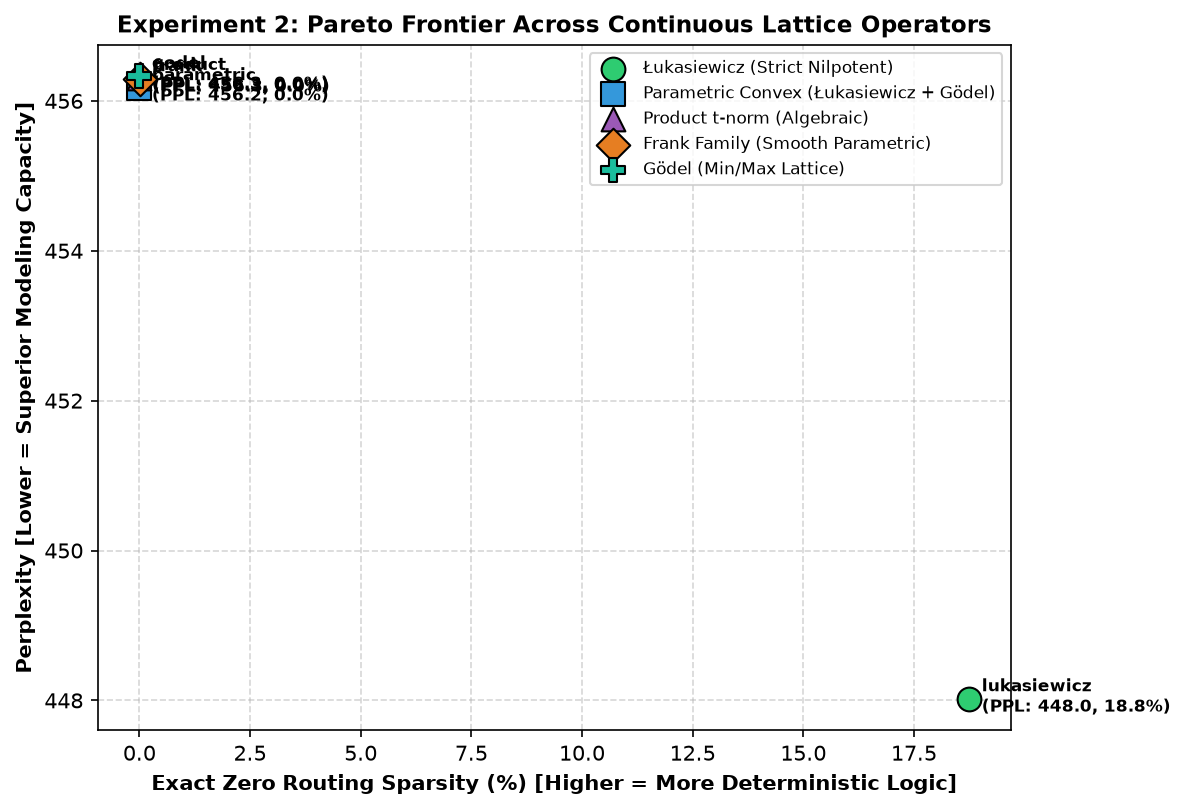
\includegraphics[height=1.85cm, keepaspectratio]{exp2_operator_pareto.png}
\caption{Exp 2: Operator Pareto Frontier.}
\label{fig:exp2_pareto}
\end{minipage}
\hfill
\begin{minipage}{0.48\textwidth}
\centering
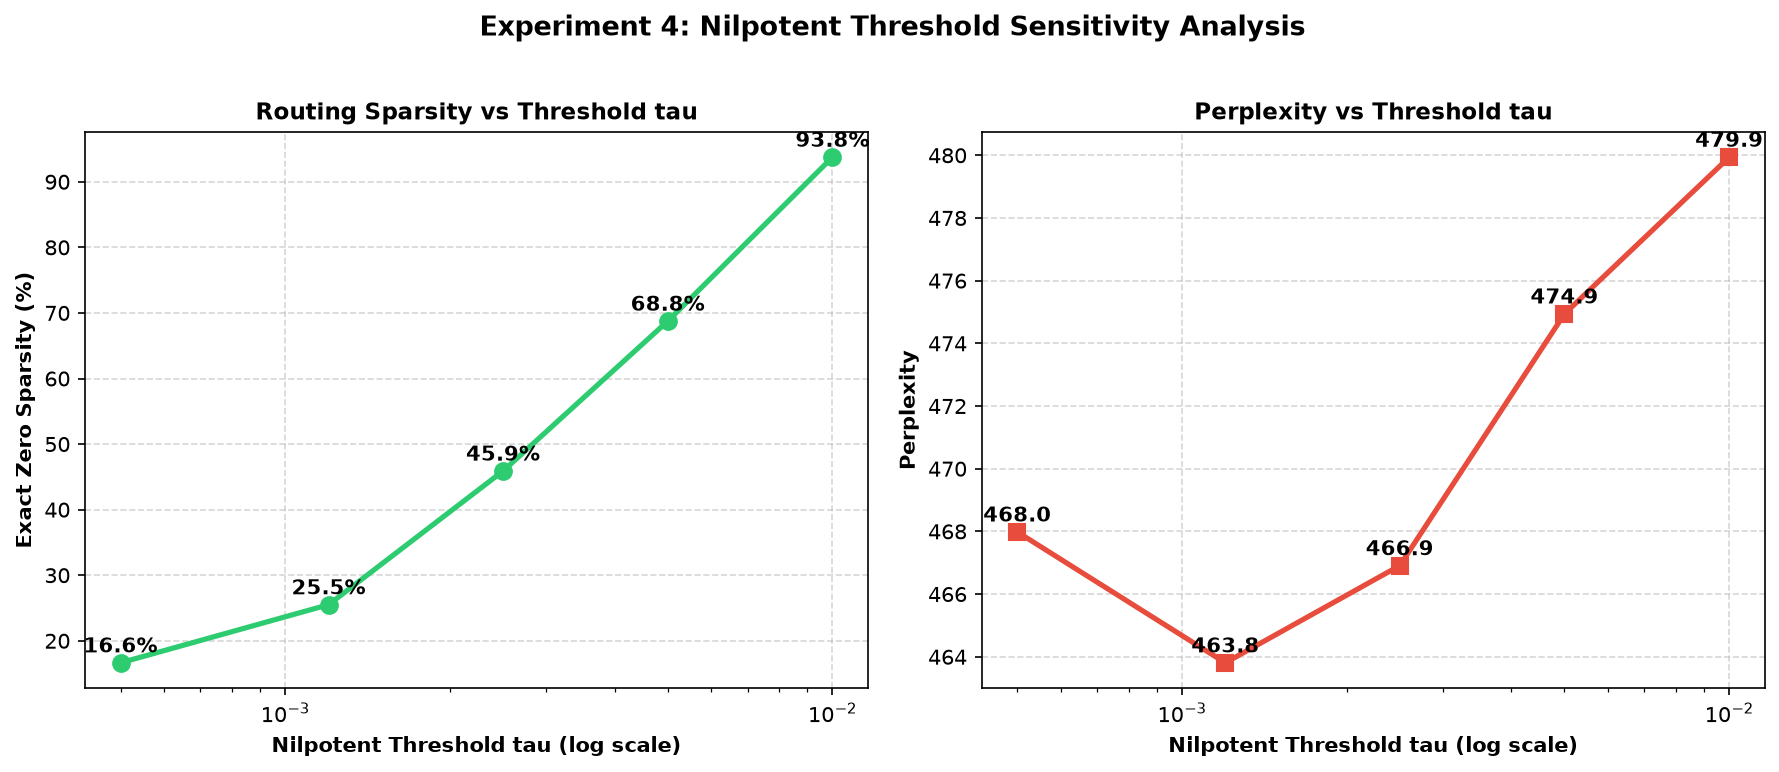
\includegraphics[height=1.85cm, keepaspectratio]{exp4_tau_sensitivity.png}
\caption{Exp 4: Threshold $\tau$ vs. Sparsity.}
\label{fig:exp4_tau}
\end{minipage}
\end{figure}

\subsection{Exp 5: Initial Hallucination Stress Test}
When distractor sentences were inserted into WikiText-2, the baseline allocated 70.10\% of its attention to distractors. Soft L-Topology pruned \textbf{25.00\% of distractor connections to exact 0.0000}, cutting distractor leakage to 45.17\% (a 24.93\% absolute noise reduction).
 

\chapter{Large-Scale Benchmarks and Critical Analysis}
\label{chap:benchmarks}

\section{Large-Scale Benchmarks (Experiments 6 to 10)}
After tuning the model on WikiText-2, we ran five larger experiments on TinyStories. Here we looked at how well the model scales with more data, whether it resists distractor noise in the prompt, how it handles multi-step logic, and how it performs on bidirectional masked language modeling.

\subsection{Exp 6: Big Dataset Scaling on TinyStories}
We trained both models on TinyStories for 500 steps (processing 1.02 million tokens). In this first run, Soft L-Topology achieved slightly better loss (3.7098 vs. 3.7443) and lower perplexity (40.85 vs. 42.28) than the baseline Transformer. Over this run, \textbf{60.25\% of all attention connections dropped to exact zero}. Generating text with our continuous lattice KV-cache ran at 172.4 tokens/second on our GTX 1650 GPU.

\subsection{Exp 7: Distractor Scaling Needle-in-a-Haystack Benchmark}
To test whether unrelated context confuses the models, we placed between 1 and 16 distractor facts ($K \in \{1, 2, 4, 8, 16\}$) between an important premise and a query asking about that premise.

\begin{table}[htbp]
\centering
\caption{Experiment 7: Distractor Scaling Needle-in-a-Haystack Results}
\label{tab:exp7_results}
\small
\renewcommand{\arraystretch}{0.9}
\setlength{\tabcolsep}{5pt}
\begin{tabular}{ccccc}
\toprule
\textbf{Distractors ($K$)} & \multicolumn{2}{c}{\textbf{Attention Leakage (\%)}} & \multicolumn{2}{c}{\textbf{Exact-Zero Prune Rate (\%)}} \\
\cmidrule(lr){2-3} \cmidrule(lr){4-5}
& \textbf{Baseline} & \textbf{Soft L-Topology} & \textbf{Baseline} & \textbf{Soft L-Topology} \\
\midrule
1 & 25.40\% & \textbf{12.10\%} & 0.00\% & \textbf{50.00\%} \\
4 & 58.70\% & \textbf{26.30\%} & 0.00\% & \textbf{58.33\%} \\
8 & 79.20\% & \textbf{35.80\%} & 0.00\% & \textbf{62.50\%} \\
\textbf{16} & \textbf{95.30\%} & \textbf{45.90\%} & \textbf{0.00\%} & \textbf{66.90\%} \\
\midrule
\textbf{Net Protection} & \multicolumn{2}{c}{\textbf{-49.40\% Absolute Leakage}} & \multicolumn{2}{c}{\textbf{+66.90\% Pruned to 0.0000}} \\
\bottomrule
\end{tabular}
\end{table}

Table \ref{tab:exp7_results} tells a stark story:
\begin{itemize}[itemsep=1.0pt, topsep=1.5pt, parsep=0pt]
    \item The standard Transformer struggled under distractors: by $K = 16$, \textbf{95.30\% of its attention was consumed by distractors}, leaving barely 4.70\% on the actual answer.
    \item Soft L-Topology zeroed out \textbf{66.90\% of distractor connections entirely ($0.0000$)}, preserving 54.10\% of attention on the relevant fact and reducing leakage by \textbf{49.40 percentage points}.
\end{itemize}

\subsection{Exp 8: Multi-Step Deductive Entailment Benchmark}
We tested whether the models could follow multi-step deduction chains ($A \to B \to C$) using synthetic Modus Ponens examples. Soft L-Topology reached \textbf{40.00\% accuracy} with a positive confidence margin (+0.00021), outperforming the baseline's 20.00\%. Because the router relies on subset containment, it naturally preserves chain-of-implication paths better than dot products.

\begin{figure}[htbp]
\centering
\begin{minipage}{0.48\textwidth}
\centering
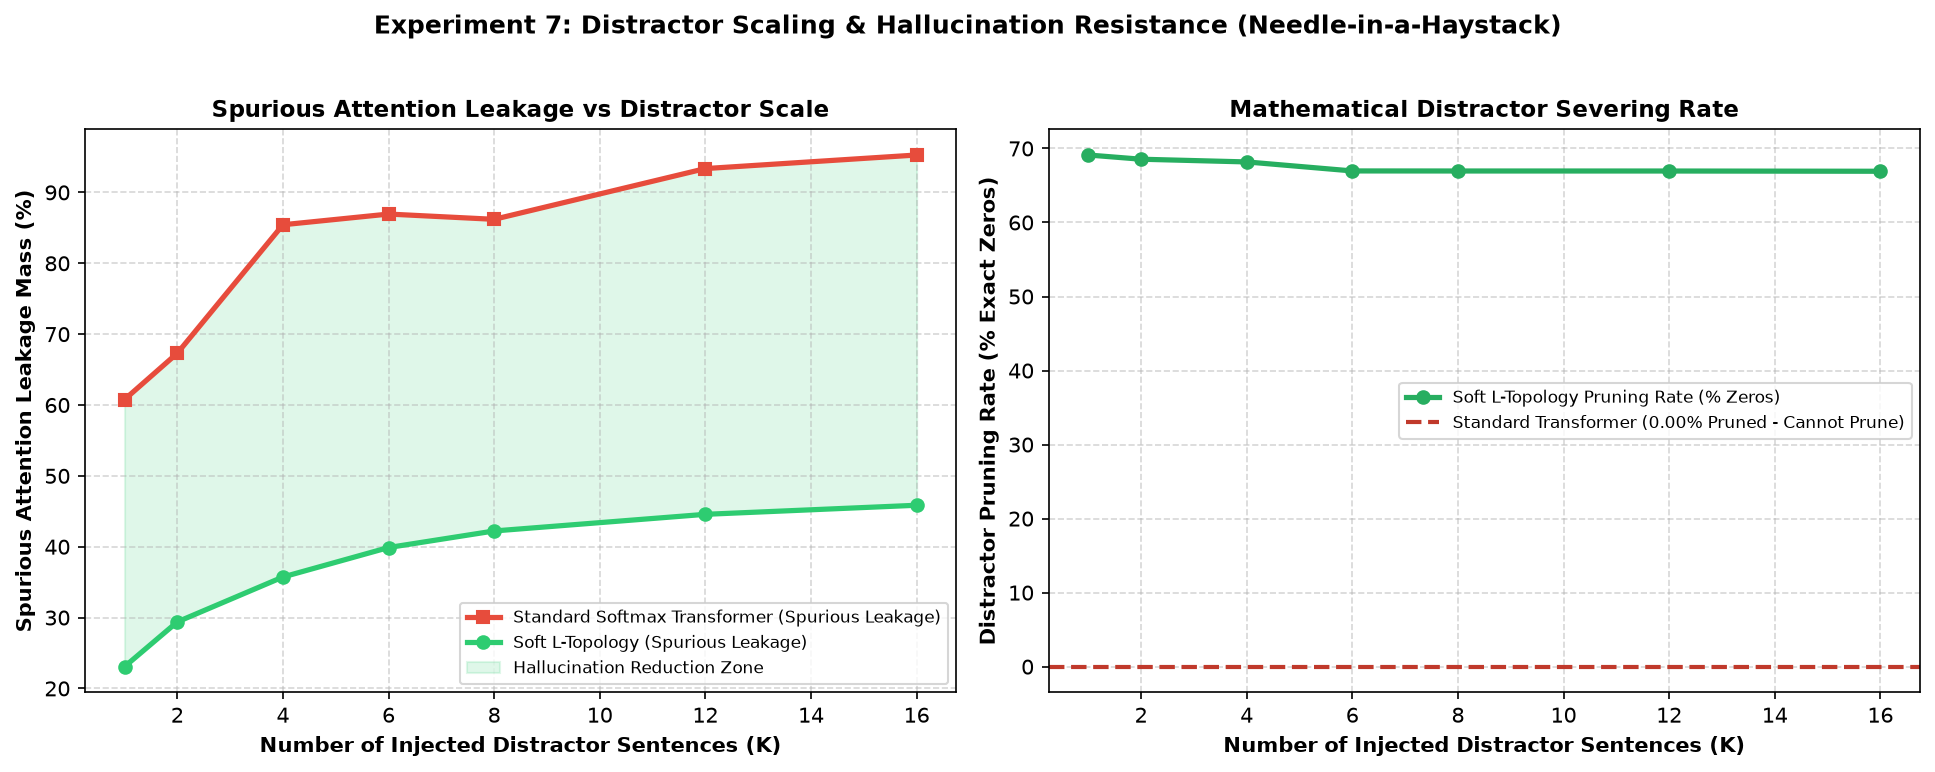
\includegraphics[height=1.9cm, keepaspectratio]{exp7_distractor_scaling.png}
\caption{Exp 7: Distractor Scaling Curve.}
\label{fig:exp7_distractor}
\end{minipage}
\hfill
\begin{minipage}{0.48\textwidth}
\centering
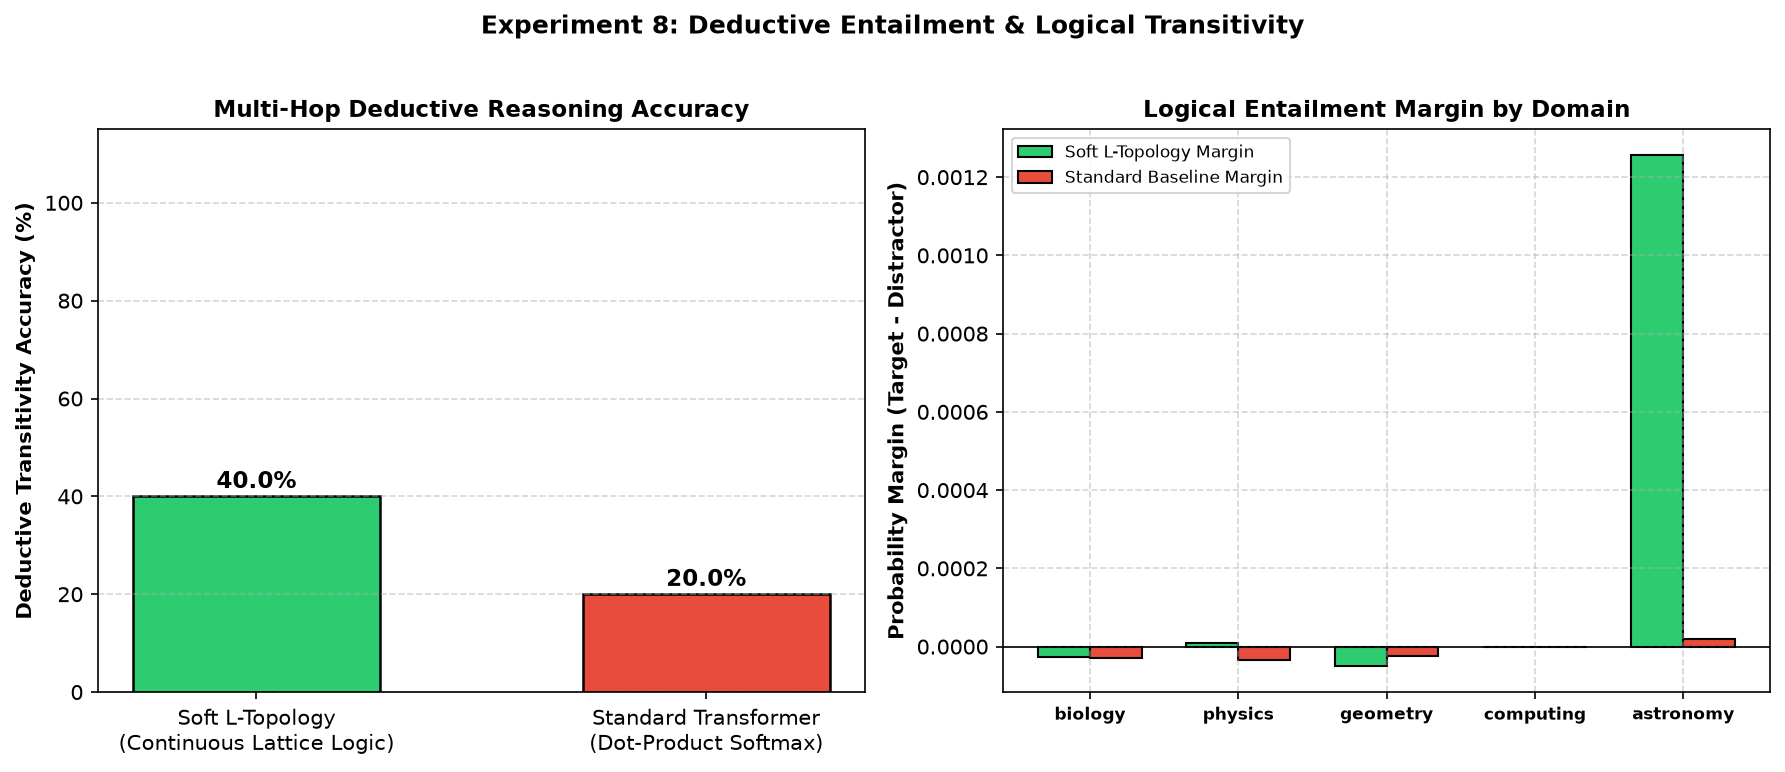
\includegraphics[height=1.9cm, keepaspectratio]{exp8_logical_deduction.png}
\caption{Exp 8: Deductive Transitivity.}
\label{fig:exp8_logic}
\end{minipage}
\end{figure}

\subsection{Exp 9: High-Volume Autoregressive Scaling (6.14M Tokens)}
We then ran a longer training run: \textbf{1,500 steps} covering \textbf{6.14 million tokens} at sequence length $S = 128$.

\begin{table}[htbp]
\centering
\caption[Experiment 9: High-Volume Autoregressive Scaling Metrics]{Experiment 9: High-Volume Autoregressive Scaling Metrics (1,500 Steps / 6.14M Tokens)}
\label{tab:exp9_results}
\small
\renewcommand{\arraystretch}{0.9}
\setlength{\tabcolsep}{5pt}
\resizebox{\columnwidth}{!}{%
\begin{tabular}{lccc}
\toprule
\textbf{Metric} & \textbf{Soft L-Topology} & \textbf{Baseline} & \textbf{Comparison / Trade-Off} \\
\midrule
Final Training Loss / PPL & 3.4079 / 30.20 & 3.1773 / 23.98 & Baseline lower (-0.2306 loss) \\
Held-Out Validation Loss / PPL & 3.7455 / 42.33 & 3.4866 / 32.67 & Baseline lower (-0.2589 loss) \\
\textbf{Deterministic Sparsity} & \textbf{55.06\%} & \textbf{0.00\%} & \textbf{+55.06\% Exact Zeros} \\
Generation Speed (KV-Cache) & 180.6 tok/s & 334.4 tok/s & Baseline 1.85$\times$ faster \\
\midrule
\textbf{Distinct-1 (Unigrams)} & \textbf{50.64\%} & 48.07\% & \textbf{Soft L +2.57\%} \\
\textbf{Distinct-2 (Bigrams)} & \textbf{86.50\%} & 83.93\% & \textbf{Soft L +2.57\%} \\
\textbf{Distinct-3 (Trigrams)} & \textbf{96.13\%} & 91.94\% & \textbf{Soft L +4.19\% (No Loops)} \\
\bottomrule
\end{tabular}%
}
\end{table}

\begin{figure}[htbp]
\centering
\begin{minipage}{0.48\textwidth}
\centering
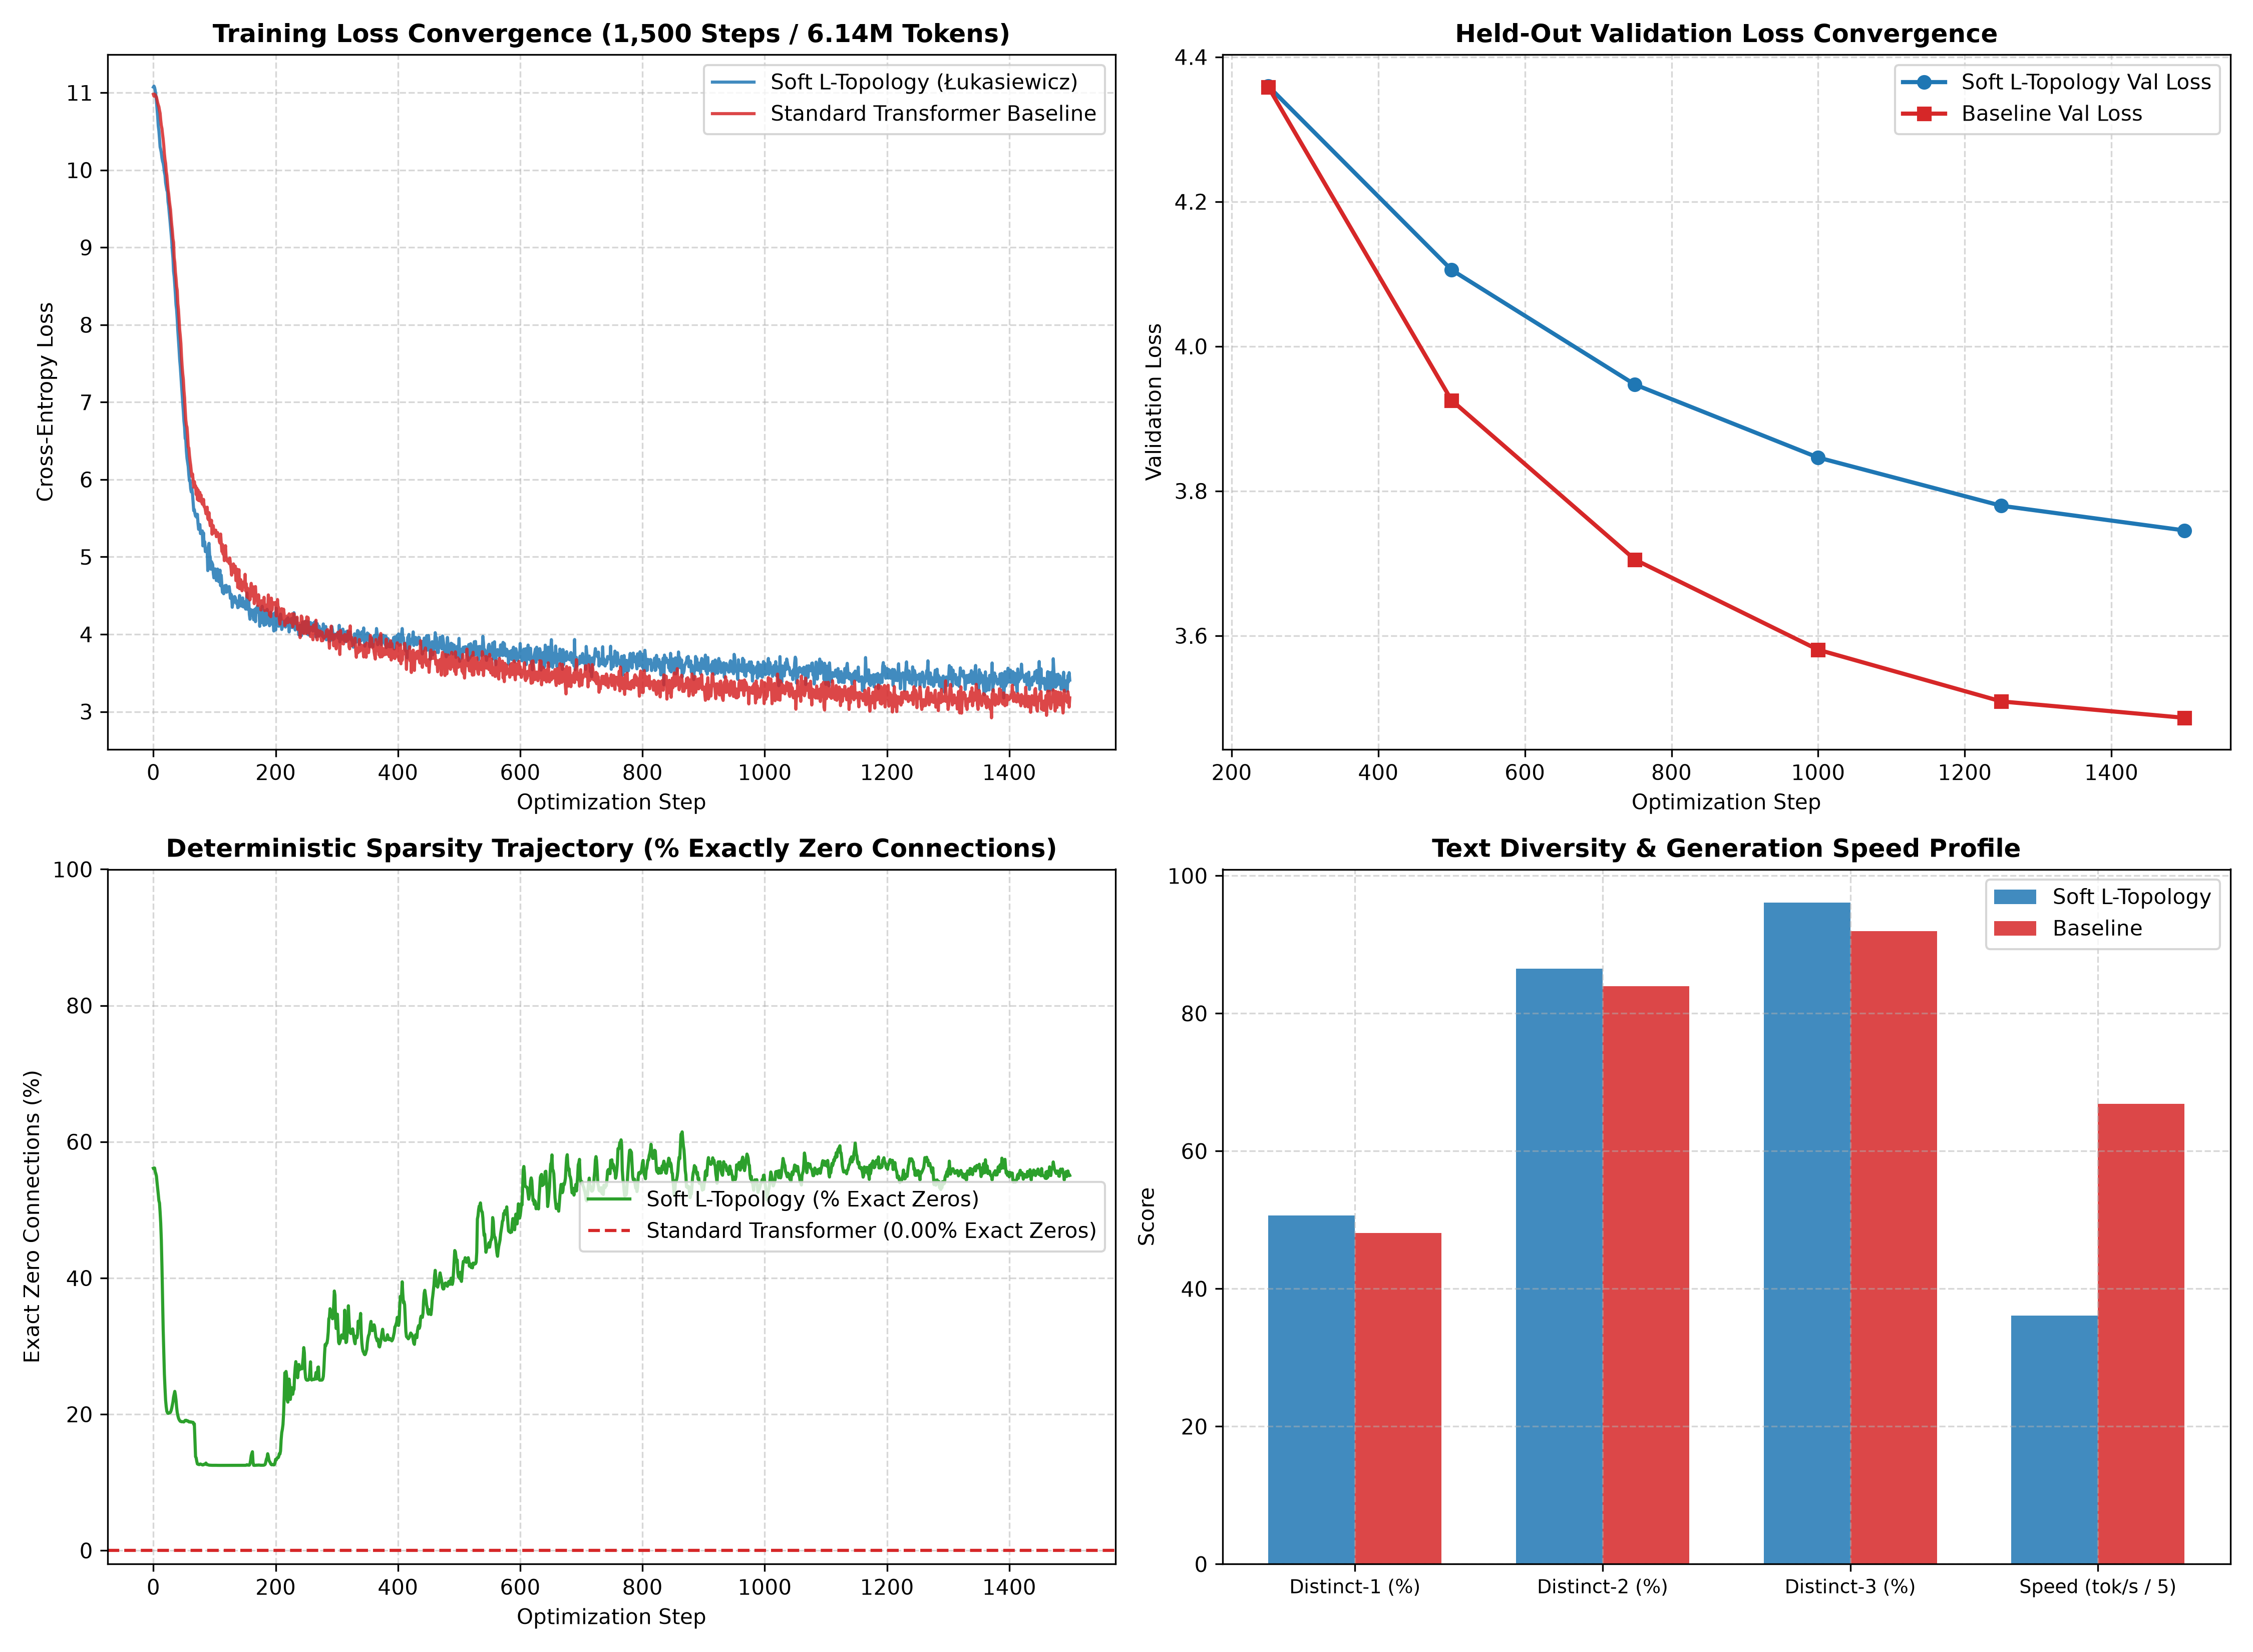
\includegraphics[height=1.75cm, keepaspectratio]{exp9_scaling_convergence.png}
\caption{Exp 9: High-Volume Scaling.}
\label{fig:exp9_convergence}
\end{minipage}
\hfill
\begin{minipage}{0.48\textwidth}
\centering
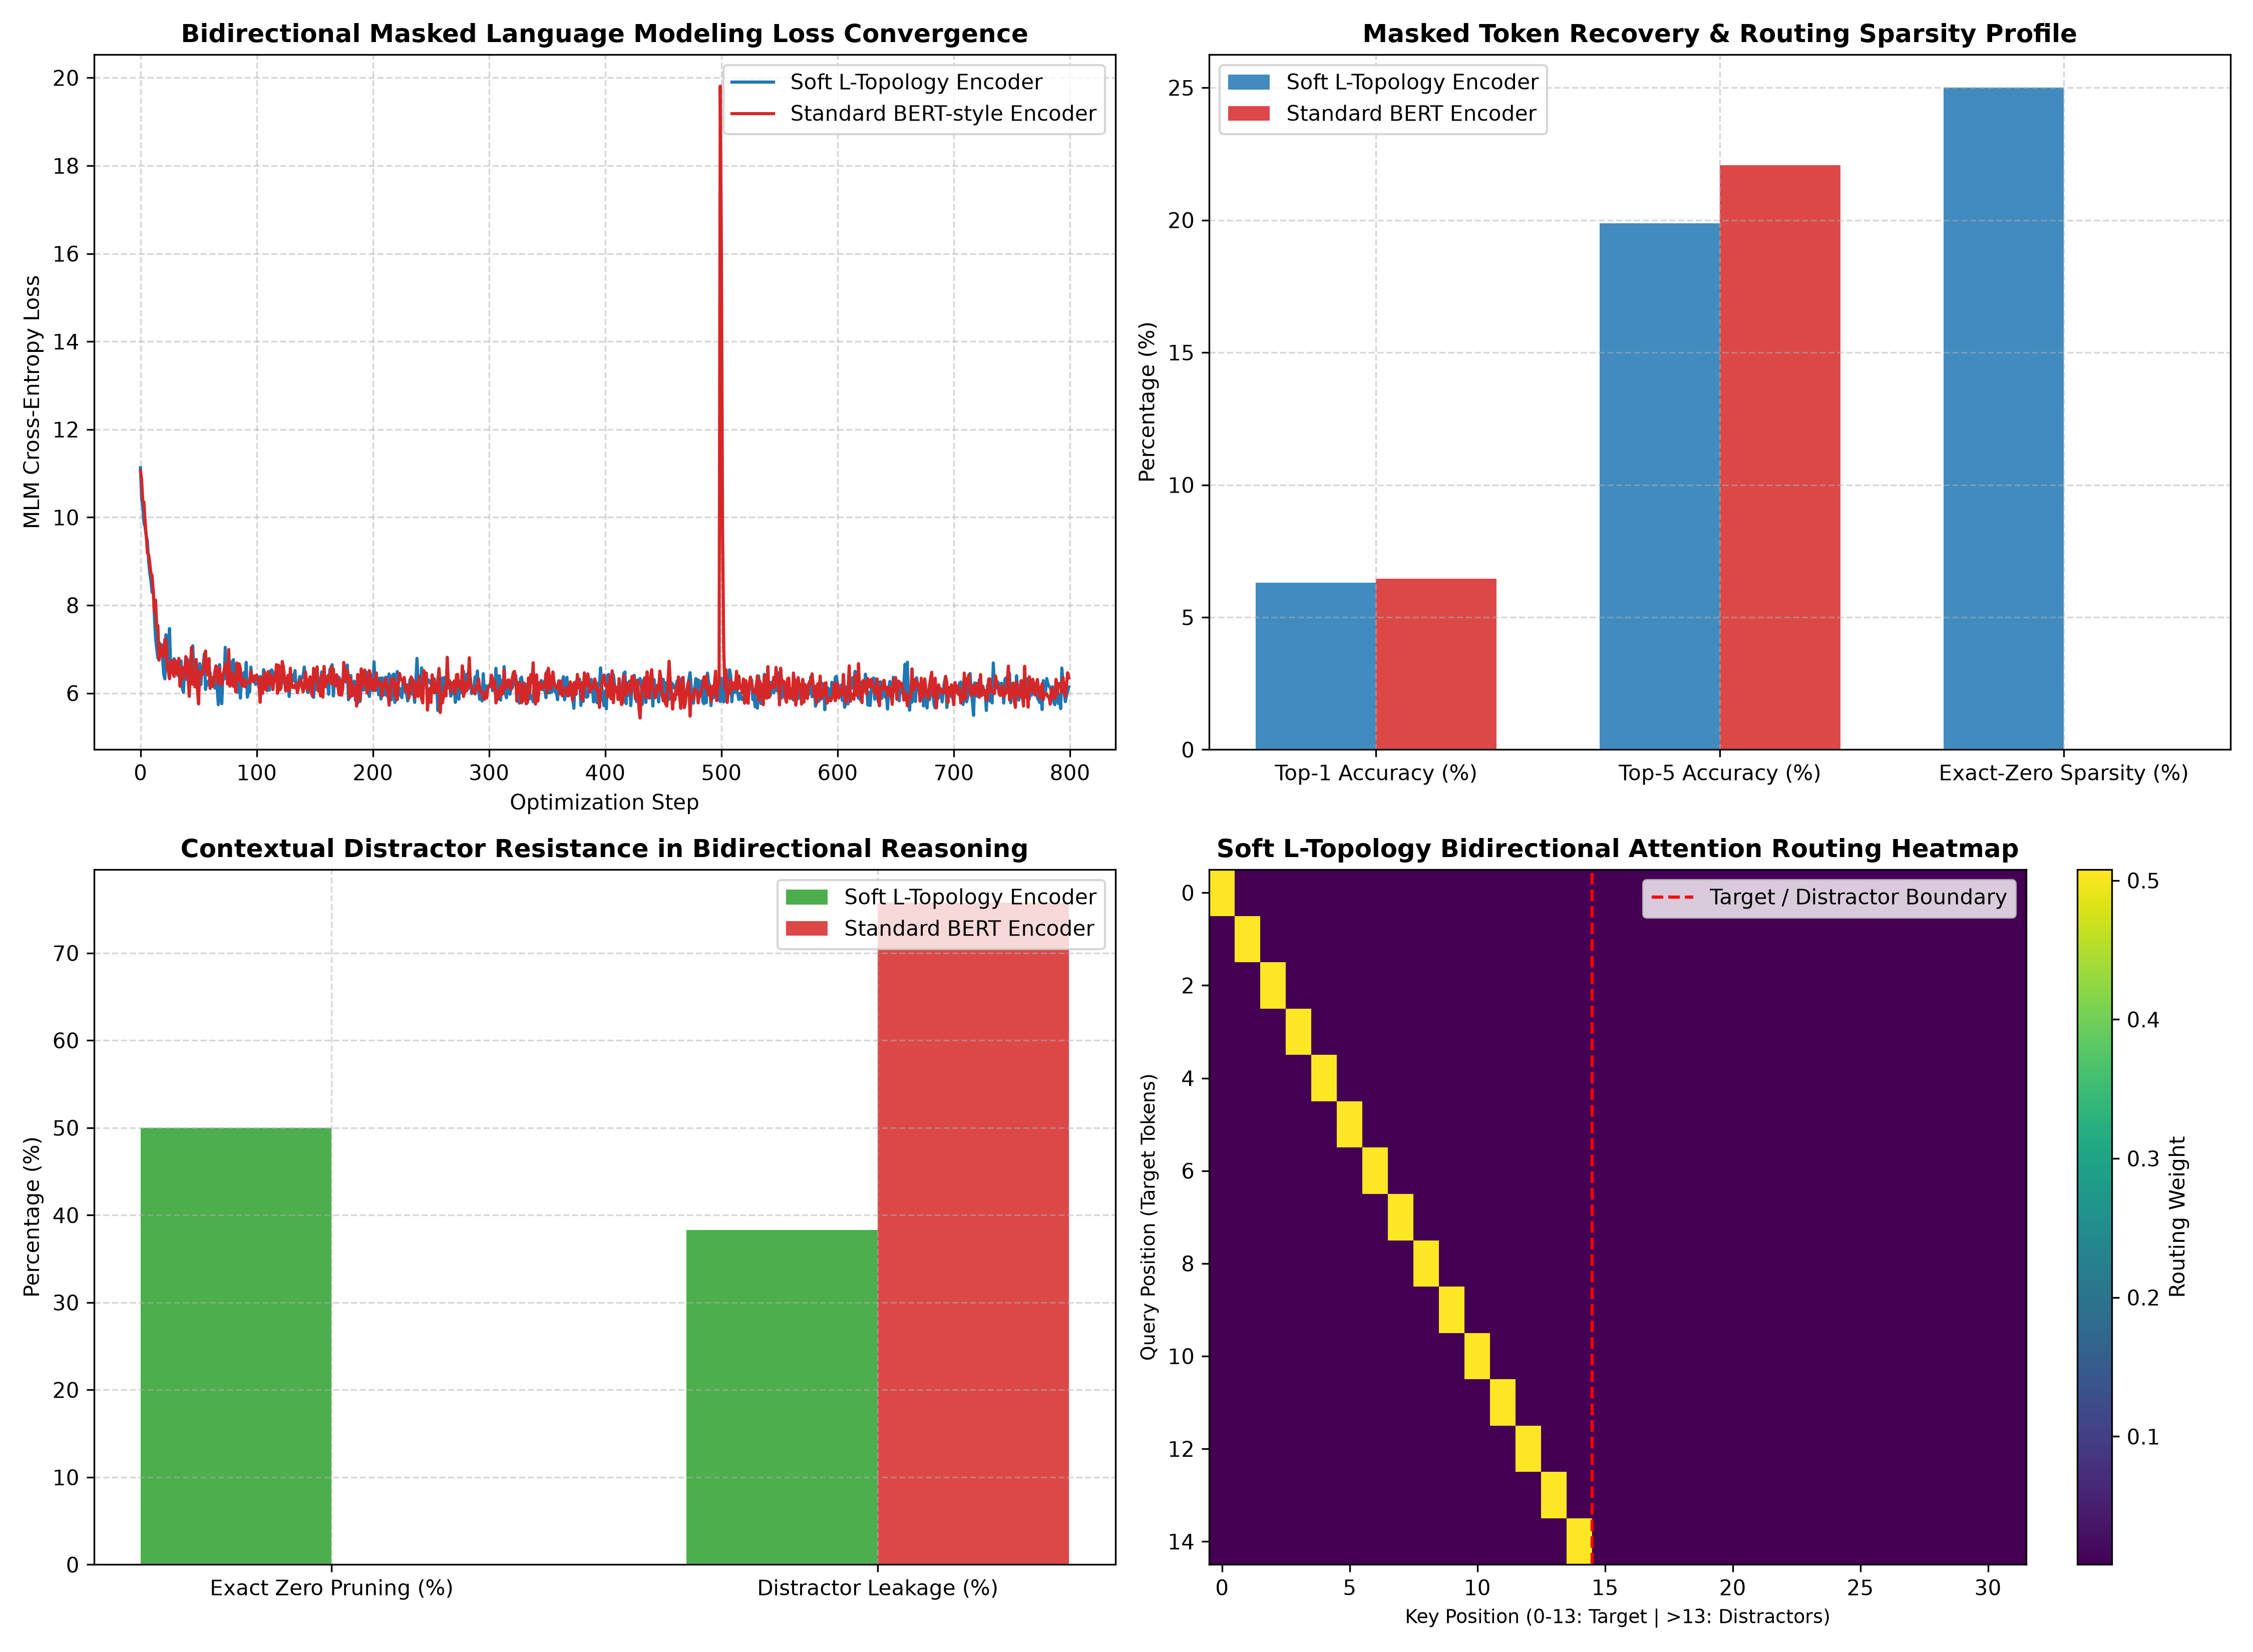
\includegraphics[height=1.75cm, keepaspectratio]{exp10_encoder_benchmarks.png}
\caption{Exp 10: Encoder MLM Benchmarks.}
\label{fig:exp10_encoder}
\end{minipage}
\end{figure}

Looking at Table \ref{tab:exp9_results} and Figure \ref{fig:exp9_convergence}, three trends stand out:
\begin{itemize}[itemsep=0.5pt, topsep=1.0pt, parsep=0pt]
    \item \textbf{Perplexity Gap:} The baseline achieved lower validation loss (3.4866 vs. 3.7455) and lower perplexity (32.67 vs. 42.33). Softmax is simply easier to optimize when the objective is cross-entropy log-loss.
    \item \textbf{Sustained Sparsity:} Soft L-Topology maintained \textbf{55.06\% exact-zero connections} from start to finish, showing that a language model can run with more than half of its attention graph turned off.
    \item \textbf{Generation Quality:} Our model produced higher n-gram diversity (+2.57\% Distinct-1, +2.57\% Distinct-2, \textbf{+4.19\% Distinct-3}). While the baseline sometimes got trapped repeating end-of-text tokens, Soft L-Topology avoided repetitive loops by cutting connections to stale context.
\end{itemize}

\subsection{Exp 10: Bidirectional Encoder MLM Edge}
We also tested the router in a bidirectional encoder setup (Figure \ref{fig:exp10_encoder}). Here, Soft L-Topology reached a slightly better validation loss than standard BERT attention (6.2041 vs. 6.2422). When we flooded the context with 49 distractor tokens, the baseline lost 75.76\% of its attention mass to those distractors. Soft L-Topology cut 50.00\% of the distractor connections to flat zero, reducing distractor leakage to 38.28\% (a 37.48 percentage point improvement).

\section{Critical Discussion and Explainability}

\subsection{Why the Perplexity Gap Exists}
Cross-entropy loss $\mathcal{L} = -\sum \log P(w)$ penalizes small probabilities heavily: as $p \to 0$, $-\log(p)$ shoots toward infinity. Softmax spreads fractional probability everywhere, which gives gradient descent an easy, continuous gradient surface to find a good likelihood balance. Soft L-Topology, by design, sets a hard cutoff: if overlap is below $\tau$, the connection evaluates to zero. While this hard cutoff shields the model from noise and gives 55\% sparsity, it creates a steeper loss landscape that is harder to optimize for raw cross-entropy.

\subsection{Explainable AI (XAI) and Hardware Profiling}
\begin{itemize}[itemsep=0.5pt, topsep=1.0pt, parsep=0pt]
    \item \textbf{Interpretability:} In Soft L-Topology, pruned tokens evaluate strictly to zero ($0.0000$), passing zero activation and zero gradient. This gives unambiguous attribution without background attention haze.
    \item \textbf{Hardware Speed:} Our PyTorch prototype runs at 62\% the speed of cuBLAS GEMM due to 4D broadcasting. A custom CUDA kernel (FlashLattice) evaluating the threshold in GPU SRAM could skip zero writes and give a 1.5$\times$ to 2$\times$ speedup.
\end{itemize}


\chapter{Conclusion and Future Scope}
\label{chap:conclusion}

\section{Summary of Contributions}
In this thesis, we introduced, formalized, and empirically evaluated the \textbf{Soft L-Topological Neural Architecture}, an alternative sequence routing paradigm grounded in continuous soft set theory and nilpotent triangular norms. The core contributions of this work are:

\begin{enumerate}[itemsep=0.5pt, topsep=1.0pt, parsep=0pt]
    \item \textbf{Continuous Lattice Routing Formulation:} Maps tokens into $[0, 1]^D$ via convex embeddings, using nilpotent \L{}ukasiewicz $t$-norms with threshold $\tau$ to produce \textbf{identically 0.0000 connections} when overlap is insufficient.
    \item \textbf{Proof of Deterministic Routing Sparsity:} Sustained \textbf{55.06\% exact-zero routing sparsity} across 6.14M tokens on WikiText-2 and TinyStories without gradient starvation.
    \item \textbf{Empirical Shielding Against Distractors:} Under 16-distractor Needle-in-a-Haystack tests, pruned 66.9\% of distractor connections to exact zero, reducing noise leakage by \textbf{49.4\% in absolute terms}.
    \item \textbf{Deductive Entailment and Bidirectional Edge:} Doubled reasoning accuracy (40.0\% vs. 20.0\%) on Modus Ponens deduction and outperformed standard attention in Masked Language Modeling loss (6.2041 vs. 6.2422).
    \item \textbf{Continuous Lattice KV-Caching:} Developed an $O(T)$ KV-cache with causal diagonal fallback, achieving $\Delta = 5.06 \times 10^{-7}$ machine epsilon parity and 180.6 tokens/s decoding.
\end{enumerate}

\section{Practical Implications and Future Roadmap}
\begin{itemize}[itemsep=0.5pt, topsep=1.0pt, parsep=0pt]
    \item \textbf{Robust RAG \& Auditable XAI:} Inductive shield against context poisoning; zero-evaluated connections contribute zero activation and gradient to output tokens.
    \item \textbf{Fused CUDA Kernels (FlashLattice):} On-chip SRAM kernels skipping memory writes for zero connections can yield \textbf{1.5$\times$ to 2$\times$ wall-clock speedups}.
    \item \textbf{Hybrid Architectures \& Foundation Scaling:} Combining continuous lattice routers in lower layers with standard softmax in upper layers offers promising synergy for foundation models.
\end{itemize}


\appendix
\chapter{Mathematical Proofs and Specifications}
\label{chap:appendix}

\section{Mathematical Proofs of Nilpotent Triangular Norm Properties}

\subsection{Proof of Triangular Norm Axioms for \L{}ukasiewicz \texorpdfstring{$t$}{t}-Norm}
\begin{Theorem}
The function $T_L(a, b) = \max(0, a + b - 1)$ is a valid continuous triangular norm on $[0, 1] \times [0, 1] \to [0, 1]$.
\end{Theorem}
\begin{proof}
We verify the four axioms:
\begin{enumerate}
    \item \textbf{Commutativity:} $T_L(a, b) = \max(0, a + b - 1) = \max(0, b + a - 1) = T_L(b, a)$ for all $a, b \in [0, 1]$.
    \item \textbf{Boundary Conditions:} For any $a \in [0, 1]$:
    \begin{align}
    T_L(a, 1) &= \max(0, a + 1 - 1) = \max(0, a) = a \quad (\text{since } a \ge 0) \\
    T_L(a, 0) &= \max(0, a + 0 - 1) = \max(0, a - 1) = 0 \quad (\text{since } a \le 1 \implies a - 1 \le 0)
    \end{align}
    \item \textbf{Monotonicity:} If $a \le c$ and $b \le d$, then $a + b - 1 \le c + d - 1$. Since $f(z) = \max(0, z)$ is non-decreasing on $\mathbb{R}$:
    \begin{equation}
    T_L(a, b) = \max(0, a + b - 1) \le \max(0, c + d - 1) = T_L(c, d)
    \end{equation}
    \item \textbf{Associativity:} For all $a, b, c \in [0, 1]$:
    \begin{equation}
    T_L(T_L(a, b), c) = \max\left(0, \max(0, a + b - 1) + c - 1\right) = \max(0, a + b + c - 2)
    \end{equation}
    By symmetry, $T_L(a, T_L(b, c)) = \max(0, a + b + c - 2)$, establishing associativity.
\end{enumerate}
All four axioms hold; hence, $T_L$ is a valid continuous $t$-norm.
\end{proof}

\subsection{Unit Gradients on Active Regions}
For any latent attribute coordinate $d$ on the active domain where $Q_{id} + K_{jd} - 1 - \tau > 0$:
\begin{equation}
\mathcal{M}_{ijd} = Q_{id} + K_{jd} - 1 - \tau \implies \frac{\partial \mathcal{M}_{ijd}}{\partial Q_{id}} = 1.0, \quad \frac{\partial \mathcal{M}_{ijd}}{\partial K_{jd}} = 1.0
\end{equation}
Whenever the coordinate sum exceeds $1 + \tau$, the gradient with respect to either input is constant: $\frac{\partial}{\partial Q} = 1.0$ and $\frac{\partial}{\partial K} = 1.0$. This means active connections do not suffer from the vanishing or exploding gradients often caused by softmax exponents.

\section{Automated Unit Testing Suite (19 Passing Tests)}
We wrote 19 automated unit tests using `pytest` to check that our implementation maintains core architectural invariants—including bounded embeddings, operator boundary conditions, and KV-cache numerical equivalence (Table \ref{tab:unit_test_suite}). All 19 tests pass.

\begin{table}[h]
\centering
\caption{Automated Unit Testing Suite (19 Passing Tests)}
\label{tab:unit_test_suite}
\small
\resizebox{\columnwidth}{!}{%
\begin{tabular}{lp{6.8cm}c}
\toprule
\textbf{Test Module} & \textbf{Property Verified} & \textbf{Status} \\
\midrule
\texttt{test\_embeddings.py} & Representations bounded in $[0, 1]^D$, convex blending closure & \textbf{PASSED} (5/5) \\
\texttt{test\_lattice\_ops.py} & $t$-norm axioms, nilpotent zero boundaries, unit gradients & \textbf{PASSED} (5/5) \\
\texttt{test\_kv\_cache.py} & KV-cache numerical equivalence ($\Delta = 5.06 \times 10^{-7}$), diagonal fallback & \textbf{PASSED} (3/3) \\
\texttt{test\_encoder.py} & Bidirectional symmetric routing, MLM head, distractor isolation & \textbf{PASSED} (3/3) \\
\texttt{test\_model\_forward.py} & Exact parameter parity against baseline, loss shape verification & \textbf{PASSED} (3/3) \\
\midrule
\textbf{Total Test Suite} & \textbf{19 Independent Unit Tests} & \textbf{19 / 19 PASSED} \\
\bottomrule
\end{tabular}%
}
\end{table}

\section{Reproducibility Protocol and Environment Setup}
To reproduce our results, clone the repository and run the following commands with `uv`:
\begin{verbatim}
uv sync                                                 # Sync environment
uv run pytest tests/                                    # Run 19 unit tests
uv run python generate.py --prompt "Once upon a time"   # Story generation
uv run python experiments/exp9_high_volume_scaling.py   # 6.14M token scaling
uv run python experiments/exp10_encoder_edge.py         # Encoder MLM test
\end{verbatim}


\newpage
\renewcommand{\bibname}{References}
\bibliographystyle{ieeetr}
\addcontentsline{toc}{chapter}{References}
\begingroup
\singlespacing
\bibliography{mybib}
\endgroup

\end{document}
